\chapter{Implementation}
Implementation is the part of SDLC in which necessary tasks are performed to put the new
system in effect.
Implementation is done after designing and coding stage. Implementation is comprised of
the involvement of the efforts of the user department, who determines that the software
is made as they wanted. The data processing department, inputs the previous data from the
system in to the new system to get the new system running. Training of staffs who would use
the system this is mostly done by conducting a training session where the system users are
instructed on how to use the system. User manual or video tutorial provide a great resource
which can later on be used by the system users when then have any query about the
system.


\section{Overview Of Programming Language Used}
\subsection{Python}
\subsection{Ruby}
\subsection{R}
\subsection{PHP}
\subsection{Java}
\subsection{Javascript}
\subsection{Luna}
\subsection{Css}


\section{Algorithms Used}


\section{Development Environment}

The development pipeline consists of three stages: development, staging and production. The development environment is a portable machine with Linux based as operative system. The source code is developed with the support of the text editor (i.e not an IDE), mainly used for its debugging and code edition features. Google Chrome is the preferred web browser, which has a built in developer tool, Chrome DevTools, highly useful to inspect HTML DOM and CSS, as well as debugging JavaScript code.

Git is used as a revision control system. The most notable characteristic of Git is its distributed system, in which each user has his own local repository where changes are committed. Only when the developer deems it convenient, the local changes are then synchronized with the remote repository, thus making them accessible to the whole team. The remote repository is hosted by GitHub, with a very interesting social networking functionality useful for future collaboration with the developer community.

In everyday’s development, Continuous Deployment technique is followed (see Figure \ref{cd-process}). Jenkins and TravisCI is used in the staging environment as a continuous deployment tool, triggering a process to deploy the system every time changes are pushed to the remote repository. This process consists of building and testing the system, running automated acceptance test and deploying the project to production once staging is stable and ready. Whenever these steps fail at some point, the process is stopped and feedback is registered in order to solve the problem.

For this to work, every new feature developed for the system should always go along with tests validating that feature. Automating these tests on a staging system allows to flawlessly merge small pieces of code with the mainline of the project at a rapid pace. The code merging also triggers a review process with all developers involved, which results in higher code quality. Besides, acceptance tests that verify the business logic can be run each time to ensure that the project requirements are met.

\begin{figure}[!h]
\center
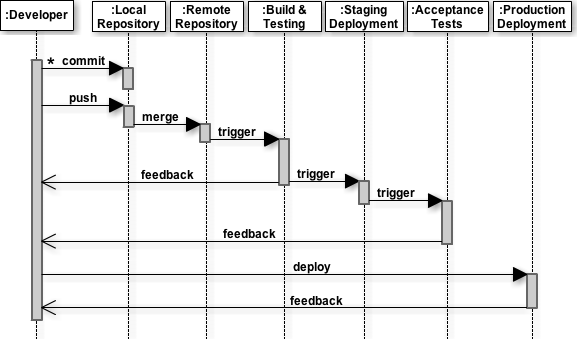
\includegraphics[keepaspectratio, width=15cm]{sequence-diagrams/cd-process.png}
\caption{Sequence diagram of the continuous delivery process}
\label{cd-process}
\end{figure}